\documentclass{article}
\usepackage[utf8]{inputenc}
\usepackage[a4paper, margin=2.5cm]{geometry}
\usepackage{graphicx}
\usepackage[french]{babel}

\usepackage[default,scale=0.95]{opensans}
\usepackage[T1]{fontenc}
\usepackage{amssymb} %math
\usepackage{amsmath}
\usepackage{amsthm}
\usepackage{systeme} %use with \system*{eq1, eq2}
\usepackage{bbm}
\usepackage{tikz-cd}

\usepackage{import}
\usepackage{xifthen}
\usepackage{pdfpages}
\usepackage{transparent}



\newcommand{\incfig}[2][1]{%
	\def\svgwidth{#1\columnwidth}
	\import{./figures_chap1/}{#2.pdf_tex}
}

\usepackage{hyperref}
\hypersetup{
	colorlinks=true,
	linkcolor=blue,
	filecolor=magenta,      
	urlcolor=cyan,
	pdftitle={Overleaf Example},
	%pdfpagemode=FullScreen,
}
\urlstyle{same} %\href{url}{Text}

\theoremstyle{plain}% default
\newtheorem{thm}{Théorème}[section]
\newtheorem{lem}[thm]{Lemme}
\newtheorem{prop}[thm]{Proposition}
\newtheorem*{cor}{Corollaire}
%\newtheorem*{KL}{Klein’s Lemma}

\theoremstyle{definition}
\newtheorem{defn}{Définition}[section]
\newtheorem{exmp}{Exemple}[section]
%\newtheorem{xca}[exmp]{Exercise}

\theoremstyle{remark}
\newtheorem*{rem}{Remarque}
\newtheorem*{note}{Note}
%\newtheorem{case}{Case}



\title{Chaîne de Markov sur un espace d'états fini}
\author{Charles Vin}
\date{2021}

\begin{document}
\maketitle



\begin{note}[]
	Il faut des bonne intuition, pas des grosse Définition on vas donc commencer pas un petit exemple pour développer l'intuition.
\end{note}

\begin{exmp}[]
	On a deux bocaux, numéros 1 et numéros 2. On pose un grain de sable dans un bocal. Il saute toute les secondes en suivant les règle suivante
	
	\begin{figure}[!htbp]
		\centering
		\incfig[0.5]{figure1}
		\caption{Chaine de Markov}
	\end{figure}

	\begin{itemize}
		\item Il démare en 1 
		\item Si il est en 1 il vas en 2
		\item Si il est en deux il vas en 1 avec une probabilité  $ \frac{2}{3} $ et donc  $ \frac{1}{3} $ d'aller en 2. 
	\end{itemize}
	Questions : 
	\begin{itemize}
		\item Sur un longue durée, il passera la moité du temps en 1 ? Plus de la moitié du temps en 2 ? Combien ? 
		\item On met 1 litre de sable en 1. Tous les grains sautent au hasard comme ci-dessus. Au bout d'un temps long, les volumes dans chaque bocal se stabilise ? Avec 1/2 litre dans chaque bocal ? Plus que 1/2 litre dans 2 ? Combien ? (même valeur qu'à la question précédente)
	\end{itemize}
\end{exmp}

\section{Rapides rappels de probabilités conditionnelles}
	$ (\omega , F, P) $ espace probabilisé \\
	\begin{align*}
		P(B|A) &= \frac{P(A \cap B)}{P(A)} \text{ si } P(A) \neq 0 \\
		P(A \cap B) &= P(B|A)P(A) \\
		P(A \cap B \cap C) &= P(C|B \cap A)P(B|A)P(A) \\
		P(D \cap C \cap B \cap A ) &= P(D|C \cap B \cap A) P(C | B \cap A) P(B|A) P(A) \\
		& \text{ect (formules des conditionnemens)} \\
		P(B) &= \sum_{i=1}^{k}P(B|A_i)P(A_i) \text{ avec } K \in N^* \text{ ou } K=\infty \text{ et } (A_i)_i \text{ partition de } \omega  
	\end{align*}

\section{Chaîne de Markov et matrice de transition}

	Une variable aléatoire représente une quantité qui dépend du hasard.
	
	Un processus stochastique (aléatoire dans un vocabulaire plus simple mdr) représente une quantité qui dépend du hasard et \textbf{du temps}. Il a la propriété de Markov si son évolution future ne dépend que de son état présent, actuel (et pas des étapes du passé).

	\begin{defn}[Propriété de Markov]
		Une suite de variable aléatoire  $ (X_n)_{n \in N} \text{ sur } (\omega , F, P)$ à valeurs dans l'ensemble fini  $ E $ est une chaine de Markov si 
		\[
			\forall n \in N, \forall e_0, e_1, ..., e_{n+1} \in E \text{ tel que } P(X_0 = e_0, X_1=e_1, ..., X_n=e_n) > 0
		.\]
		\[
			P(X_{n+1} = e_{n+1} | X_n = e_n, X_{n-1}=e_{n-1}, ..., X_0=e_0) = P(X_{n+1} = e_{n+1}|x_n=e_n)
		.\]
		
		\begin{note}[]
			Ici n représente le temps. La propriété de Markov dit bien que la proba du future ne dépend pas du passé
		\end{note}
		
		Ceci s'appelle la \textbf{propriété de Markov}.  $ E $ est \textbf{l'espace d'états}. Dans ce cours, on suppose $ E $ fini. Ici on le munis de la tribut de les partie de $ E $ : $ P(E) $ 		
	\end{defn}

	\begin{exmp}[]
		Les deux bocaux \\
		\begin{itemize}
			\item $E={1,2}$ ensemble des bocaux = espace d'états
			\item $ \displaystyle X_n $ : Position du grain de sable à l'instant n
			\item $ \displaystyle X_0 = 1 $ : On démare dans 1
			\item $ \displaystyle P(X_1=2) = 1$
			\item $ \displaystyle P(X_2=1 | X_1 =2) = \frac{2}{3}, P(X_2=2 | X_1=2) = \frac{1}{3} $ 
			\item $ \displaystyle P(X_4=2 | X_3=2, X_2=1,X_1=2,X_0=1) = \frac{1}{3} = P(X_=2 | X_3 = 2)$
		\end{itemize}
	\end{exmp}

	\begin{exmp}[Marche aléatoire réfléchie dans $\{-N, ..., N\}$\\]
		Espace d'état : $ \{-N, -N+1, ..., N-1, N\} $ $\rightarrow$ $2N+1$ position possible. A chaque pas, on tire à pile ou face si on va à gauche ou à droite en partant d'une position initiale $ X_0=0 \text{ ou } X_0 = e_0$ fixé.

		\begin{figure}[!htbp]
			\centering
			\incfig[0.5]{figure2}
			\caption{}
			\label{}
		\end{figure}

		$ p \in ]0,1[ $ proba d'aller à droite fixée, $ X_n $ position après n pas 
		\begin{align*}
			P(X_{n+1}=e_{n+1} | X_n = e_n, ..., X_0=e_0) &= \systeme*{
				p \text{ si } e_n = {-N, ..., N-1},
				0 \text{ si } e_n = N
			} \\
			P(X_{n+1}=e_{n+1} | X_n = e_n, ..., X_0=e_0) &= \systeme*{
				{1-p} \text{ si } e_n = {-N+1, -N+2 ..., N}, 
				0 \text{ si } e_n = -N
			} \\
			\text{fin de chaine : }& \\
			P(X_{n+1}=e_{n+1} | X_n = N, X_{x-n} = e_{n-1}, ..., X_0=e_0) &= p \\
			P(X_{n+1}=e_{n+1} | X_n = -N, ..., X_0=e_0) &= 1-p
		\end{align*}
		\begin{note}[]
			J4AI PAS COMPRIS 
		\end{note}
		
		
	\end{exmp}
	
	\begin{exmp}[Problème de la ruine du joueur]
		On joue à pile ou face contre un adversaire. On gagne 1€ si on fait pile (proba $ p \in ]0,1[ $). On perd 1€ si on fait face. On commence avec $ k $ € et notre adversaire à $ N-k $. Le jeu s'arrête quand l'un n'a plus d'argent. \\
		Quelle est la probabilité que l'on finisse ruiné ?

		\begin{itemize}
			\item On a bien une chaîne de Markov sur $ \{0, 1, 2, ..., N\} $. 
			\item $ X_n $  : La fortune du joueur à l'instant $ n $. $X_0 = k$
			\item  $ P(X_{n+1} = 0| X_n = 0) = 1 $, $ P(X_{n+1} = 0 | X_n = N) = 1 $ : Le jeu s'arrete lorsque l'un des joueurs est ruiné.
			\item $ P(X_{n+1} = e+1 | X_n = e) = p $ si $ e \in \{1,2,...,N-1\} $   
			\item $ P(X_{n-1} = e-1 | X_n = e) = 1-p $ si $ e \in \{1,2,...,N-1\} $   
		\end{itemize}
	\end{exmp}

	\begin{defn}[Chaine de Markov homogène]
		On dit que la chaine de Markov $ (X_n)_{n \in N} $ est \textbf{homogène} si 
		\[
			\forall n \in N, \forall e,e' \in  E, P(X_{n+1} = e' | X_n = e) = P(X_1 = e' | X_0 = e)
		.\]

		\begin{note}[]
			aka quand les proba sur les flèches du graph ne change pas avec le temps. Si c'est la même proba qu'au début
		\end{note}
		
		Dans ce cas, la probabilité de transition de $ e $ vers $ e' $ est : 
		\[
			\pi (e,e') = P(X_{n+1} = e' | X_n = e) 
		.\]
		Elle ne dépend pas de n. 

		En numérotant les états $ E = {e_1, e_2, ..., e_{card(E)}} $ on fabrique la \textbf{matrice de transition} qui à la ligne $ i $  colonne $ j $  la probabilité $ \pi (e_i,e_j) $ d'aller en $ e_j $ quand on est en $ e_i $. On peut aussi représenter les probabilités de transition sur un graphe
	\end{defn}

	\begin{exmp}[bocaux]
		$ E=\{1,2\}, \pi =  
		\begin{pmatrix}
			0 & 1 \\
			\frac{2}{3} & \frac{1}{3}
		\end{pmatrix}$
		\begin{note}[]
			Proba d'aller en 1 depuis 1 = 0, proba d'aller en 2 depuis 1 = 1, proba d'aller en 1 depuis 2 = 2/3, proba d'aller en 2 depuis 2 = 1/3
		\end{note}
	
		\begin{proof}
			\begin{align*}
				\forall e \in E, \sum_{e' \in E}^{} \pi (e, e') = \sum_{e' \in E}^{} P(X_1 = e' | X_0 = e) &= P(\bigcup_{e' \in E} \{X_1=e'\} | X_0 = e) \\
				&= P(X_1 \in E | X_0 = e) \\
				&= P(\omega | x_0 = e ) = 1 
			\end{align*}
		\end{proof}
	\end{exmp}
	\begin{exmp}[Matrice de transition de la marche aléatoire]
		\begin{figure}[!htbp]
			\centering
			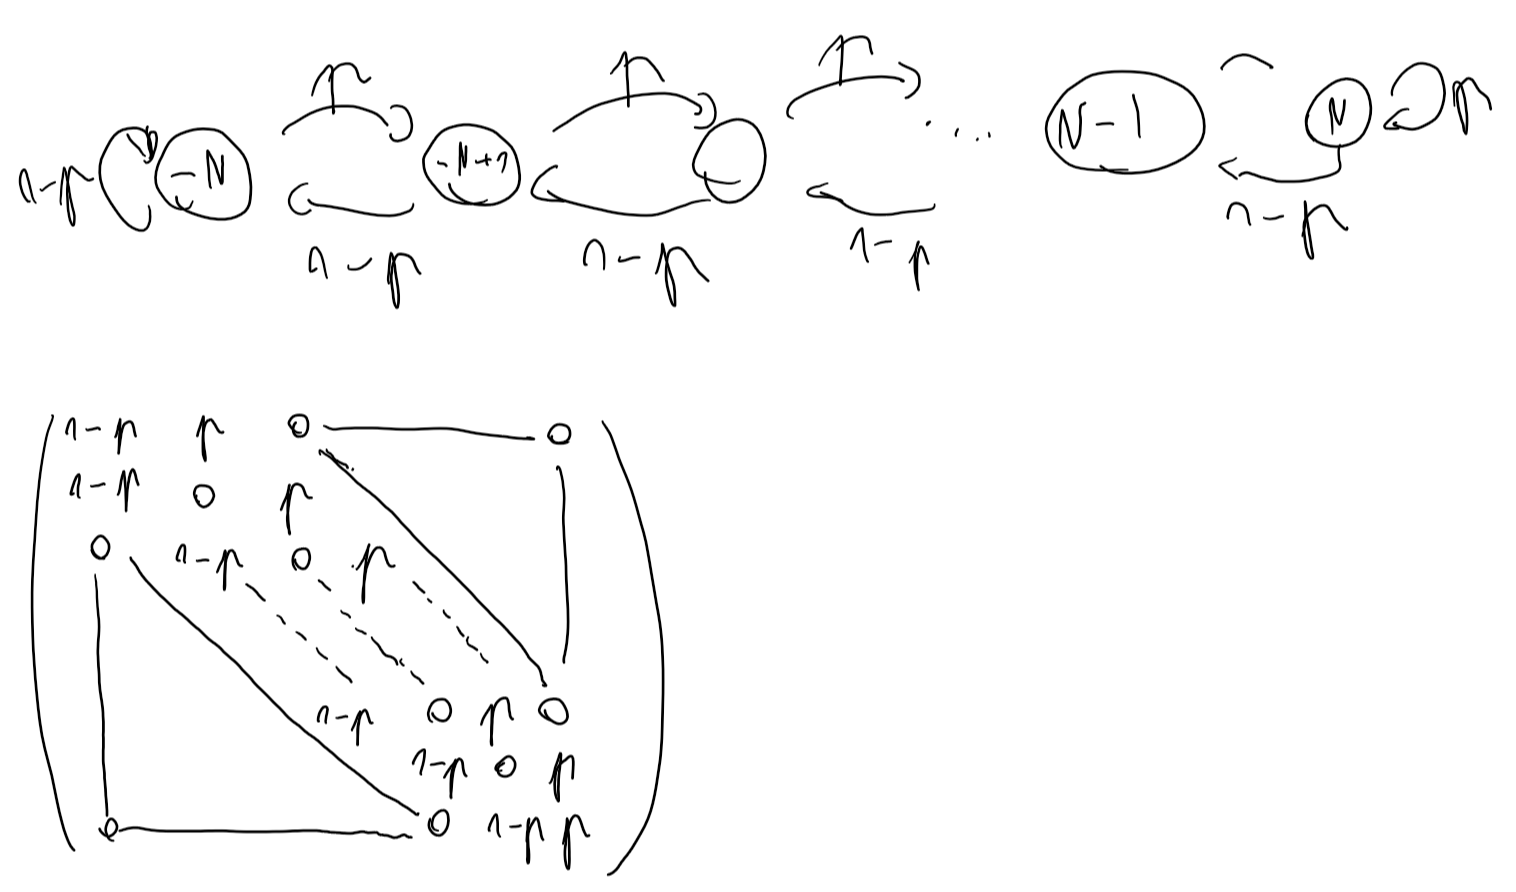
\includegraphics[width=0.75\textwidth]{./figures_chap1/figure3.png}
			\caption{Matrice de transition de la marche aléatoire}
			\label{graph1}
		\end{figure}
		Voir Figure \ref{graph1}.
	\end{exmp}

	\begin{exmp}[Matrice de transition de la ruine du joueur]
		\begin{figure}[!htbp]
			\centering
			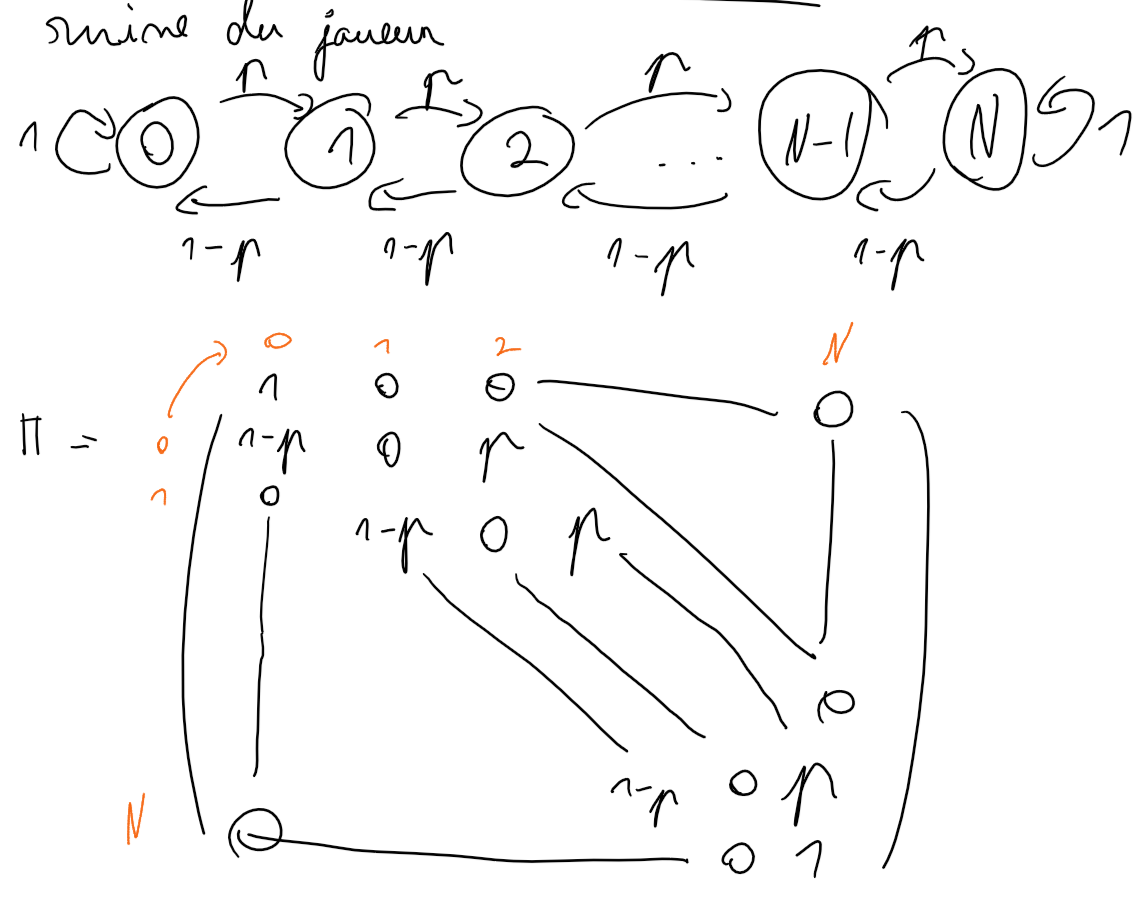
\includegraphics[width=0.75\textwidth]{./figures_chap1/figure4.png}
			\caption{Matrice de transition de la ruine du joueur}
			\label{graph2}
		\end{figure}
		Voir Figure \ref{graph2}.
	\end{exmp}
	
	\section{Trajectoire et évolution en loi}
	A partir d'ici, on a $ (X_n)_{n \in N} $ chaine de Markov homogène de matrice de transition $ \pi  $ . 

	Pour chaque $ \omega \in \Omega$ , la suite $X_0(\omega), X_1(\omega ), ... , $ s'appelle une trajectoire.
	
	\begin{thm}[]
		\begin{align*}
			\forall n \in N, \forall e_0, e_1, ..., e_n \in E \\ 
			P(X_0 = e_0, X_1=e_1, ..., X_n=e_n) &= P(X_0= e_0) \pi (e_0,e_1) \pi (e_1, e_2) ... \pi (e_{n-1}, e_n) \\
			&= P(X_0 =e_0) \prod_{i=1}^{n} \pi (e_{i-1}, e_i)
		\end{align*}
	\end{thm}
	\begin{note}[]
		On fait comme en proba discrète : on multiplie les probas
	\end{note}
	
	
	\begin{proof}
		\begin{align*}
			P(X_n=e_n, x_{n-1}=e_{n-1}, ... X_0 = e_0)
			&= P(X_n=e_n |X_{n-1} = e_[n-1, ..., X_0=e_0]) \\
			&\rightarrow P(X_n =e_n | X_{n-1} = e_{n-1}) = \pi (e_{n-1}, e_n) \\
			&= P(X_{n-1} = e_{n-1} | X_{n-2} = e_{n-2}, ... ,X_0=e_0)\\
			&\rightarrow P(X_{n-1} = e_{n-1} | X_{n-2} = e_{n-2}) = \pi (e_{n-2, e_{n-1}}) \\
			&= ... \\
			&= P(X_1 = e_1 | X_0=e_0)P(X_0 = e_0) \rightarrow \pi (e_0,e_1) P(X_0=e_0)
		\end{align*}
		\begin{note}[]
			J'ai pas giga bien écrit la preuve pas le time mais t'as capté.
		\end{note}
	\end{proof}	
	
	
Cours du 9/14/2021

La loi à l'instant n (la loi de $ X_n $ ) est : 
\begin{align*}
	\mu _n &= (P(X_n = e_1), P(X _{n} = e _{n} , ... P(X _{n} = e _{Card E}))) \\ 
	&= \mu_n (e_1), \mu_n (e_2)
\end{align*}

Quand E est fini $ \mu _n = (P(X_n p e_i))_{i \in E } $  forme un vecteur ligne.

\begin{thm}[]
	$ \forall n \in  N, \mu _{n+1} = \mu _{n} \pi  $ et $ \mu _{n} = \mu _0 \pi ^n $
	\begin{note}[]
		$ \mu _{n+1}   $ dit comment on passe de l'état n à n+1
	\end{note}

	\begin{proof}[]
		La i ème coordonnée du vecteur ligne $ \mu _{n} \pi  $  est : 
		\[
			(\mu _{n} )(e_i) = \sum_{e \in E}^{} \mu _{n} (e) \pi (e,e_i) = \sum_{e \in E}^{}P(X _{n} = e) P(X _{n+1} = e_i | X _{n} =e) = P(X _{n+1} = e_i	) = \mu  _{n+1} (e_i)
		.\]
	\end{proof}
\end{thm}

\begin{exmp}[]
	Exemple des deux bocaux \\
	\begin{itemize}
		\item $ \mu _0 = (1,0) $ 
		\item $ \mu _1 = (0,1) = \mu _0 \pi  $ 
		\item $ \mu _2 = (0,1) \big(\begin{smallmatrix}
			0 & 1\\
			2/3 & 1/3
		\end{smallmatrix}\big) = (\frac{2}{3}, \frac{1}{3})$ 
		\item $ \mu _3 =  (\frac{2}{3}, \frac{1}{3}) \big(\begin{smallmatrix}
			0 & 1 \\
			2/3 & 1/3
		\end{smallmatrix}\big) = (\frac{2}{9}, \frac{7}{9})$
		\item $ \mu _4 = \mu _3 \pi = \mu _0 \pi ^4 =  (\frac{2}{9}, \frac{7}{9}) \big(\begin{smallmatrix}
			0 & 1 \\
			2/3 & 1/3
		\end{smallmatrix}\big) = (\frac{14}{27}, \frac{13}{27})$  
	\end{itemize}
\end{exmp}

\begin{rem}[]
	$ P(X _{n+k} = e' | X_n = e) = \pi ^k (e,e') $ est le coeff ligne e colonne e' de $ \pi ^k $. 
	\begin{proof}[]
		Si la propriété est vraie pour $ k-1 $. On vas faire une récurence. 
		\begin{align*}
			\Omega = \bigcup_{x \in E} \{X _{n+k-1} =x=  \} \\
			P(X _{n+k} &= e' | X_n = e) = \sum_{x \in E}^{} P(X _{n+k} = e' , X _{n+k-1} = x | X_n = e) \\
						&= \sum_{x \in E}^{} \frac{P(X _{n+k} = e' , X _{n+k-1} = x, X_n = e)}{P(X _{n+k-1} = x, X _{n} =e )} * \frac{P(X _{n+k-1} n X_n = e)}{P(X_n = e)} \\
						&= \sum_{x \in E}^{} P(X _{n+k} = e' | X _{n+k-1} = x, X _{n} =e) P(X _{n+k-1} = x | X_n = e) \\
						&= \sum_{x \in E}^{} \pi (x, e') \text{ (par la prop de Markov)} * \pi ^{k-1} (e,x) \text{ (par hypothèse de récurence)}
		\end{align*}
	\end{proof}
	\begin{note}[]
		BRO WTF 
	\end{note}
\end{rem}

\section{Récurence, transience, périodicité}

\begin{defn}[]
	L'état $ e' $ est \textbf{accessible} depuis l'état $ e $  si la chaine a une probabilité strictement positive d'aller en $ e' $ quand elle est en $ e $ (en une ou plusieurs étapes). 
	\[
		\exists k \in N , \pi ^k(e,e') > 0
	.\]
	ou 
	\[
		\exists k \in N, \exists e_1, e_2, ... e_{k-1}, \pi (e,e_1)\pi (e_1,e_2), ... , \pi (e_{k-2}, e_{k-1}) \pi (e_{k-1}, e') > 0
	.\]
	
	\begin{note}[]
		Il existe un chemin en k étape pour aller de e à e' strictement positive. \\ ou 
		Il existe un chemin tel que on a une probabilité strictement positive de faire le premier chemin, ect, jusqu'au dernier
	\end{note}
	
	Quand c'est accessible depuis e et e accessible depuis e', on dit que $e$ et $e'$ sont \textbf{communiquant}. \\
	Si $ e $ et $ e' $ communiquant, et $ e' $  et $ e'' $ communiquent, alors $ e $  et $ e'' $ communiquent. Donc on peut partitionner $ E $ en classes d'éléments qui communiquent entre eux. On dit que la chaine est \textbf{irréductible} si tous les états communiquent 
\end{defn}

\begin{exmp}[]
	Les deux bocaux \\
	Ca se lit sur un graph : est-ce que 1 est accessible depuis 2 ? oui lol . Est-ce que 2 est accessible depuis 1 ? oui aussi $\rightarrow$ tout le monde communiquent c'est irréductible
\end{exmp}

\begin{exmp}[]
	Fil d'attente \\
	3 personnes font la queue à l'ouverture d'un guichet. Le temps qu'on s'occupe d'une personne (2 min), il y a une chance sur deux qu'une autre arrive. On vas faire le graph
	\begin{figure}[!htbp]
		\centering
		\incfig[0.5]{figure5}
		\caption{Fil d'attente}
		\label{}
	\end{figure}
	$\begin{pmatrix}
		1/2 & 1/2 & 0 & 0 \\
		1/2 & 1/2 & 0 & 0 \\
		0 & 1/2 & 1/2 & 0 \\
		0 & 0 & 1/2 & 1/2
	\end{pmatrix}$	
\end{exmp}

\begin{exmp}[]
	Marche aléatoire \\
	C'est communiquant en 1 noyaux $\rightarrow$ irréductible
\end{exmp}

\begin{exmp}[]
	Ruine du joueur \\
	O et 1 sont seul, et le reste communique 
\end{exmp}

\begin{exmp}[]
	Voir Figure \ref{exm_no_name}
	\begin{figure}[htbp]
		\centering
		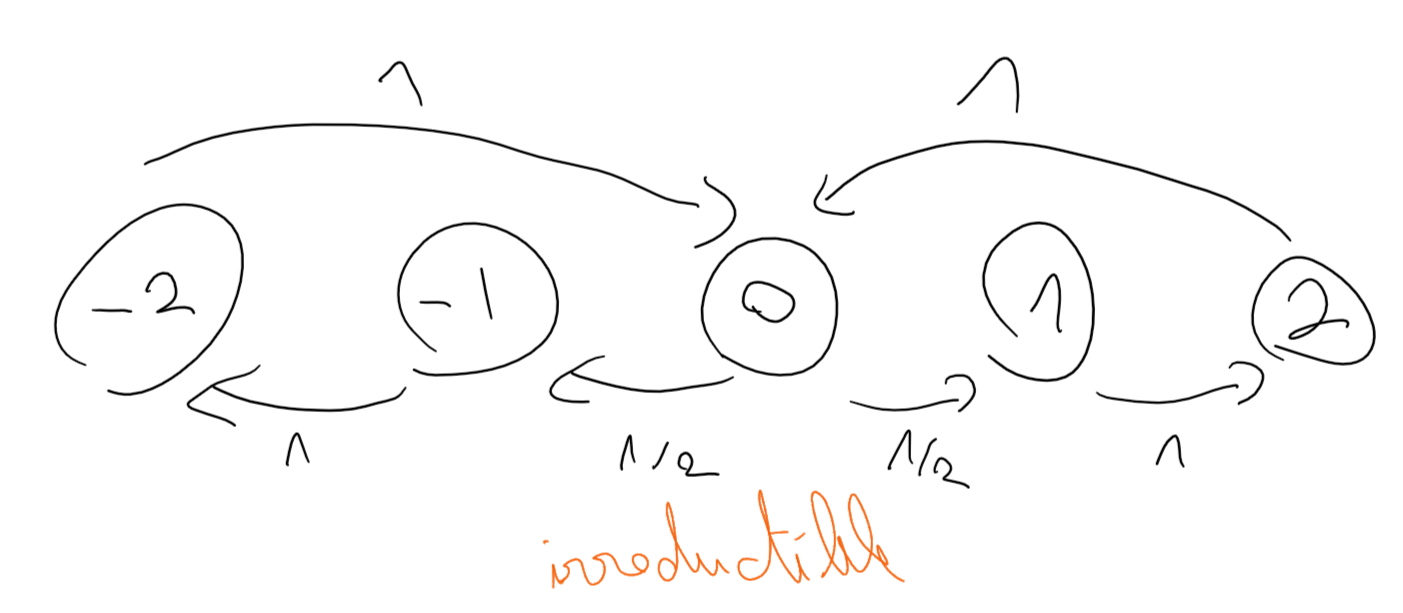
\includegraphics[width=.5\textwidth]{figures_chap1/figure6.png}
		\caption{Exemple sans nom}
		\label{exm_no_name}
	\end{figure}
\end{exmp}

\begin{defn}[Absorbant]
	Un état est \textbf{absorbant} si $ P(X_1 = e| X_0 = e) = 1 $
\end{defn}

\begin{defn}[Récurrent]
	Un état $ e \in E $ est \textbf{récurent} si partant de $ e $ , on finit toujours par y revenir : 
	\[
		P(\exists n \in N, X_n =e | X_0 = e) = 1
	.\]
	Si un état n'est pas récurrent, on di qu'il est \textbf{transient}
	Voir Figure \ref{recurent}
	\begin{figure}[htbp]
		\centering
		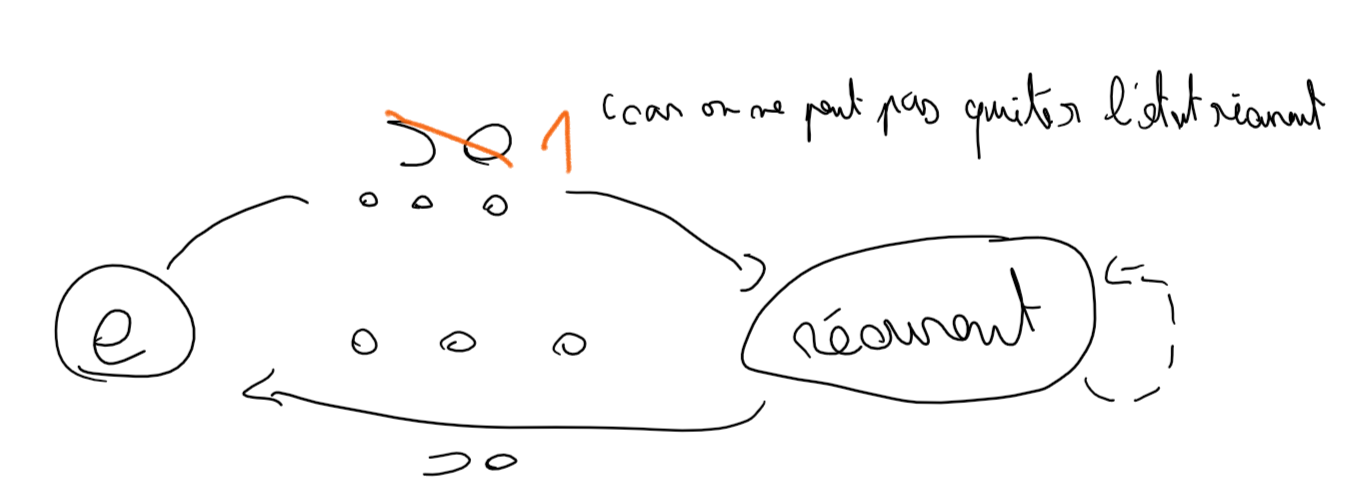
\includegraphics[width=.5\textwidth]{figures_chap1/figure7.png}
		\caption{Graph avec récurence}
		\label{recurent}
	\end{figure}
\end{defn}
\begin{thm}[]
	Sur ces définitions \\
	\begin{itemize}
		\item Partant d'un état récurrent, on y passe une infinité de fois.
		\item Un état qui communique avec un état récurrent est toujours récurrent.
		\item Un état qui communique avec un état transient est toujours transient.
	\end{itemize}
\end{thm}

\begin{exmp}[]
	Tout nos exemples : \begin{itemize}
		\item LEs deux bocaux : Tout le monde est récurent
		\item Fil d'attente : La classe récurente : \begin{itemize}
			\item La classe O, 1 est récurente
			\item La classe 2 et la classe 3 sont transient 
		\end{itemize}
		\item Marche aléatoire : Tout le monde est récurrent 
		\item Ruine du joueur : \begin{itemize}
			\item La classe 0 et la classe 1 sont Récurent et Absorbant
			\item La classe 1 à n-1 est transient
		\end{itemize}
		\item Dans l'exemple sans nom de onenote (voir Figure \ref{exm_no_name}) : Tout le monde es récurent;

	\end{itemize}
\end{exmp}

\begin{thm}[]
	Quand l'espace d'état $ E $ est fini, il y a toujours au moins un état récurrent. Donc si la chaine est irréductible, tout les états sont récurrents.
	\begin{note}[]
		Si c'est infinie, on peut imaginer quelque chose qui s'en vas loin à l'infinie
	\end{note}
\end{thm}

\begin{defn}[]
	La période d'un état $ e \in E $, c'est le PGCD des temps de retour possible en $ e $ . 
	\[
		d(e) = PGCD(\{k \geq 1, \pi ^k (e,e) > 0\})
	.\]
	\begin{note}[]
		Temps de retour possible = On part de e pour aller en e en un nombre k d'étape. On peut faire plein de détour.
		En combien d'étape je peux faire pour partir de e et renvenir en e
	\end{note}
	Si $ d(e) = 1 $ , on dit que $ e $ est \textbf{apériodique}	 
\end{defn}

\begin{thm}[Admise]
	Les états qui communiquent entre eux ont tous la même période.
\end{thm}

\begin{exmp}[]
	Nos exemples habituel \begin{itemize}
		\item Des 2 bocaux : \begin{itemize}
			\item $ d(2) = PGCD(\{1,2,3,...\}) = 1$
			\item $ d(1) = PGCD(\{2,3,4,5,...\})= 1 $  
		\end{itemize}
		Elle est donc irréductible et apériodique.
	\item File d'attente : \begin{itemize}
		\item $ d(3) = d(2) =1 $
		\item $ d(0) = d(1)= 1 $  
	\end{itemize}
	\item Marche aléatoire : \begin{itemize}
		\item $ d(0) = PGCD(\{2,4,6,..., 2N, 2N+1, 2N+2\}) $
		\item On fait des aller retour basique au début $\rightarrow$ nombre paire 
		\item Puis quand on arrive au bous, il y a la boucle $\rightarrow$ les nombres impaires arrivent
	\end{itemize}
	\item Ruine du joueur : \begin{itemize}
		\item $ d(0) = d(N) = 1 $
		\item $ d(1) = d(2) = ... = d(N-1) = 2 $  
	\end{itemize}
	\item Exemple sans nom : \begin{itemize}
		\item Période 3
		\item $ d(0) = PGCD (\{3,6,9,12, ..., \})=3 $ 
	\end{itemize}
	\end{itemize}
\end{exmp}

\section{Invariance, réversibilité, convergence, ergodicité}
\begin{defn}[]
	La chaine de Markov de matrice de transition $ \pi  $. Elle admet $ \mu  $ comme mesure invariante/stationnaire si $ \mu \pi = \mu  $ 
	\begin{note}[]
		Si $ \mu _0 \pi = \mu _1$ alors $ \mu _1 \pi = \mu _2$ ect \\
		$ \mu  $ donne une quantité, il mesure. Pour une mesure invariante, si on prend une photo à un instant t, ça sera la même photo à l'instant t+1.
	\end{note} 
	$ \mu $ est une mesure \textbf{réversible} si 
	\[
		\forall e, e' \in E, \mu (e) \mu (e,e') = \mu (e') \pi (e',e)
	.\]
	Ce qui va de e à e' = ce qui va de e' à e \\
	Si $ \sum_{e \in E}^{} \mu (e) = 1 $ on parle de probabilité réversible ou invariante 
\end{defn}

\begin{exmp}[]
	Nos exemples habituelle : \begin{itemize}
		\item Les deux bocaux : Si on est à la répartiton $ \mu  $. $ \mu(1)$ représente la quantité dans le bocal 1, same pour 2. \\ A l'étape suivante, la quantité qui va de 1 à 2 est $ \mu (1) * \pi (1,2)$ et celle qui vas de 2 à 1 est $ \mu (2)\pi (2,1) $ .
		\item  
	\end{itemize}
\end{exmp}

\begin{prop}[]
	Toute mesure réversible est invariante. 
\end{prop}

\begin{proof}[]
	Si $ \mu  $ est réversible : $ \displaystyle (\mu \pi)(e) = \sum_{x \in E}^{}\mu (x) \pi (x,e) =_{\text{réversibilité}} = \sum_{x \in E}^{} \mu (e) \pi (e,x) = \mu (e) \sum_{x \in E}^{} \pi (e,x) = 1$  
\end{proof}

\begin{rem}[]
	Les lois limites sont invariantes \\
	Si $ \displaystyle \mu _{n} \rightarrow_{n \rightarrow + \infty } \mu  $, comme $ \mu _{n+1}  = \mu _{n}  \pi  $ donc $ \mu = \mu \pi $
\end{rem}
\begin{prop}[admis]
	Une chaine irréductible sur un espace d'état fini admet une unique probabilité invariante.
\end{prop}

\begin{note}[Rappel Loi des grands nombres]
	$ X_i $ i.i.d 
	\[
		\frac{1}{n}\sum_{i=1}^{n}X_i \longrightarrow ^{Proba}_{n \to + \infty } E(X_1)
	.\]
	Convergence en probabilité
	\[
		\Leftrightarrow \forall \epsilon > 0 P(\left| \frac{1}{n} \sum_{i=1}^{n}X_i - E(X_1)\right| > \epsilon)
	.\]
	COnvergence en loi : 
	\[
		V_n \to _{n \to \infty } ^{loi} V_{\infty} \text{ si } F_{v_n} \to F{V_{\infty }}(t), \forall t \text{ where } F_{V_{\infty}} \text{ est continue }
	.\]
	On exquive les sauts 
\end{note}



\begin{thm}[Théorème de convergence en loi (admis)]
	Une chaine de Markov $ (X_n)_{n \in N} $ \textbf{homogène irréductible apériodique} sur un espace d'état fini $ E $ converge en loi vers son unique probabilité invariante $ \mu  $ au sens où  : \\
	Pour tout état initiale $ e_0 \in E $ 
	\[
		\forall e \in E , \lim_{n \to \infty} P(X_n = e | X_0=e_0) = \mu (e)
	.\]
	\begin{note}[]
		Ne dépend pas du point de départ, au bout d'un certain temps la chaine oublie d'ou elle est partie.
	\end{note}
	Conséquence : Pour toute loi initiale $ X_0 \sigma \mu _0 $ 
	\begin{align*}
		P(X_n = e) &= \sum_{e_0 \in E}^{} P(X_n = e | X_0 = e_0) P(X_0 = e_0) \\
					& \longrightarrow _{n \to + \infty } \sum_{e_0 \in E}^{}\mu (e) \mu_0(e_0) = \mu (e)
	\end{align*}
	Convergence en loi : 
	\[
		F_{X_n}(t) = p(X_n \leq t) = \sum_{e \leq t ,e \in E}^{}P(X_n = e) \longrightarrow _{n \to  \infty } \sum_{e \leq t, e \in E}^{}\mu (e) = F_\mu (t)
	.\]
\end{thm}

\begin{thm}[Ergodique]
	(Loi forte des grands nombres pour les chaines de Markov homogènes irréductible) \\ 
	Soit $ (X_n)_{n \in N} $ une chaine de MArkov homogène irréductible de probabilité invariante $ \mu  $ sur l'espace d'état fini $ E $. \\ 
	Pour toute $ f:E \rightarrow R $ 
	\[
		P(\lim_{n \to \infty} \frac{1}{n} \sum_{k=0}^{n} f(X_k) = \sum_{e \in E}^{}f(e)\mu (e)) = 1
	.\]
	\[
		\Leftrightarrow \frac{1}{n}\sum_{k=0}^{n}f(X_k) \longrightarrow ^\text{presques surement}_{n \to \infty } \sum_{e \in E}^{}f(e)\mu (e)
	.\]
	i.e la moyenne en temps converge vers la moyenne en espace (espace des états) \\
	En particulier, pour tout état $ e \in E $ 
	\[
		\frac{1}{n}\sum_{k=0}^{n}\mathbbm{1}_{X_k=e} \longrightarrow _{n \to \infty }^{p.s.} \sum_{e' \in E}^{}f(e')\mu (e') = \sum_{e' \in e}^{}\mathbbm{1}_{e' = e}\mu (e') = \mu (e)
	.\]
	Proposition de temps passé dans l'état $ e $ entre les instants $ 0 $ et $ n $ converge vers la mesure stationnaire prise dans l'état $ e $.
\end{thm}
\begin{exmp}[des deux bocaux]
	Je cherche si dans mon graph avec les deux bocaux j'ai une mesure stationnaire. Le graph est irréductible et apériodique. Par Théorème il existe une seule valeur stationnaire $ mu \pi = \mu $. \\
	$ \mu (a,b) , a=\mu (1), b=\mu (2), \pi \big(\begin{smallmatrix}
		0 & 1 \ \
		2/3 & 1/3
	\end{smallmatrix}\big)$  
	\[
		\mu \pi = \mu \Leftrightarrow \systeme*{
			\frac{2}{3}b=a, 
			a + \frac{1}{3}b = b
		} \Leftrightarrow \systeme*{
			a= \frac{2}{3}b, 
			a+b = 1 \text{ car } \mu \text{ est une probabilité}
		}		
	.\]
	\[
		\frac{2}{3}b + b = 1 \Leftrightarrow b=\frac{3}{5}, a=\frac{2}{5}
	.\]
	La probabilité invariante : $ \mu = (\frac{2}{5}, \frac{3}{5}) $ \\
	\begin{note}[]
		Si on revient longtemps plus tard, on a 2/5 de chance que le grain de sable soit dans le bocal 1 et 3/5 pour le bocal 2. \\
		Cela dit aussi pour un seul grain quelle proportion de temps il a passé dans le bocal 1 et 2.
	\end{note}
	\[
		\mu (1) \pi (1,2) = \frac{2}{5} * 1
	.\]
	\[
		\mu (2) \pi (2,1) = \frac{3}{5} * \frac{2}{3} = \frac{2}{5}
	.\]
	$ \mu  $ est réversible car c'est égal	
\end{exmp}
\begin{exmp}[Fil d'attente]
	\begin{figure}[!htbp]
		\centering
		\incfig[0.5]{figure5}
		\caption{Fil d'attente}
		\label{}
	\end{figure}
	Non irréductible. On cherche $\mu$ invariant, un probabilité invariante ? Si oui 
	\[
		\mu (a,b,c,d), \pi = \begin{pmatrix}
			1/2 & 1/2 & 0 & 0 \\
			1/2 & 1/2 & 0 & 0 \\
			0 & 1/2 & 1/2 & 0 \\
			0 & 0 & 1/2 & 1/2
		\end{pmatrix}
	.\]
	\[
		\systeme*{
			\frac{1}{2}a + \frac{1}{2}b = a,
			\frac{1}{2}a + \frac{1}{2}b + \frac{1}{2}c = b,
			\frac{1}{2}c + \frac{1}{2}d = c,
			\frac{1}{2}d = d,
			a+b+c+d = 1
			}
		\Leftrightarrow
		\systeme*{
			a =b
			c=0
			d=0,
			a+b+c+d = 1
			}
		\Leftrightarrow
		\mu = (\frac{1}{2}, \frac{1}{2}, 0, 0) \text{ invariante}
	\]
	
	\begin{align*}
		& \text{Pour la paire \{0,1\}: } \mu (0) \pi (0,1) = \frac{1}{4} = \mu (1) \pi (1,0) \\
		& \text{Pour la paire \{1,2\}: } \mu (1)\pi (1,2) = \frac{1}{2}*0 = \mu (2) \pi (2,1) = 0 \text{ Idem pour \{1,3\}, \{0,3\}, \{2,3\}, \{0,2\}}
	\end{align*}
\end{exmp}

\begin{exmp}[] 
	Exemple sans nom \\

	% https://tikzcd.yichuanshen.de/#N4Igdg9gJgpgziAXAbVABwnAlgFyxMJZABgBpiBdUkANwEMAbAVxiRAFoBGEAX1PUy58hFJ3JVajFm3YAmXvxAZseAkVnjq9Zq0QhiCgSuFEAzJsk623PkaFqUAFgvbpe+TwkwoAc3hFQADMAJwgAWyQxEBwIJDIQACMYMCgkU3iGOiSGAAVBVREQBhhAnBAtKV0QG0UQ8LjqGKQNROTUxHSKqz0aoNCIxGdo2MQWpJSkdk7LN2ryoqyYXPyTPWCsHwALMtsQOoGWpo7qcfap+NcqzgB6eWpM7LzjBxB1rZ3a-rTGkaHTyeml2s8weSye9kKb22hj2X1GP0iJzaaQulWst14FB4QA
	\begin{tikzcd}
		-1 \arrow[rr, "1", bend left] & -2 \arrow[l, "1", bend left] & 0 \arrow[r, "1/2"', bend right] \arrow[l, "1/2", bend left] & 1 \arrow[r, "1"', bend right] & 2 \arrow[ll, "1"', bend right]
	\end{tikzcd}

	irréductible période 3, $ \mu =(\frac{1}{6}, \frac{1}{6}, \frac{2}{6}, \frac{1}{6}, \frac{1}{6}), \mu \pi = \mu  $, la période empêche la convergence 
\end{exmp}

\end{document}
